\section{Introduction}
\label{sec:intro}

Over five centuries ago, Albrecht D\"urer contributed two enduring landmarks at the intersection of mathematics and the visual arts: the order-four magic square in his 1514 engraving \emph{Melencolia~I} (square \#175 in Fr\'enicle's 1693 census of the $880$ order-four magic squares \cite{frenicle1693,dudeney1917amusements,andrews1960magic}) and the first printed polyhedral net unfoldings in his 1525 treatise \emph{Underweysung der Messung} \cite{durer1525underweysung,shephard1975convex,demaine2007geometric,ghomi2014durer}. Recall that an arrangement $S=(s_{ij})_{0\le i,j<n}$ of the integers $\{1,\dots,N\}$, $N=n^2$, is a \emph{semi-magic square} if every row and column sums to the magic constant $\mu_n=n(N+1)/2$, and a \emph{magic square} if the two main diagonals also sum to $\mu_n$. Measuring coordinates from the board centre and the mean entry $\bar s=(N+1)/2$,
\begin{equation}
\label{eq:coords}
x_j = j - \frac{n-1}{2},\qquad
y_i = \frac{n-1}{2} - i,\qquad
z_{ij} = s_{ij} - \frac{N+1}{2},
\end{equation}
turns each cell $(i,j)$ into a three-dimensional point and radial vector from the origin $O=(0,0,0)$:
\[
\mathbf p_{ij}(\lambda) = (x_j,\, y_i,\, \lambda z_{ij}) \in \R^3,\qquad
P_S(\lambda) = \bigl\{\mathbf p_{ij}(\lambda) : 0\le i,j<n\bigr\},
\]
where $\lambda>0$ is the vertical lift scale (\Cref{fig:origin-vectors-3d}(a)). The convex hull
\[
\mathcal G_\lambda(S) := \conv P_S(\lambda) \subset \R^3
\qquad\bigl(\mathcal G(S):=\mathcal G_1(S)\bigr)
\]
is a three-dimensional convex polyhedron that we call the \emph{Magic Gem} of $S$, reuniting D\"urer's magic squares with his polyhedral geometry.

In classical work on the planar mechanics of magic squares, Loly \cite{loly2004invariance} and Rogers and Loly \cite{rogers2004inertia,rogers2005multipole} interpreted the entries $s_{ij}$ as point masses on the flat grid $\mathbf r_{ij}=(x_j,y_i)$, proving that the planar centre of mass lies at the origin $O$ and that the polar moment of inertia $\sum_{i,j}s_{ij}(x_j^2+y_i^2)=n^2(n^4-1)/12$ is invariant across all semi-magic squares of order $n$. Inspired by fabricating physical 3D-printed models, radial balance wheels, ball-and-rod wireframes, interconnected strut sculptures, and folded cardstock cutouts in the open-source \texttt{magicGemWeb} studio \cite{mathewson2025magicgemweb}, this paper investigates one unifying physical and sculptural question across dimensions:

\begin{quote}
\itshape
When a magic square is lifted into $\R^3$ and fabricated as a physical sculpture---whether as a $16$-spoke radial star or weighted balance wheel from the origin (\Cref{sec:vectors}), a kinetic spinning top on a central pivot (\Cref{sec:dynamics}), a cast solid, nested two-material core, 3D-printed wireframe, complete $K_{16}$ strut network, or folded papercraft shell (\Cref{sec:nested}), or a freestanding column of stacked blocks (\Cref{sec:stacking})---when does the combinatorial balance of the magic square translate into physical equilibrium, smooth rotation, and structural stability?
\end{quote}

\Cref{fig:hero-squares} introduces the six flagship order-four magic squares (\#175, \#70, \#45$\leftrightarrow$\#54, \#46, \#673, and \#763$\leftrightarrow$\#756) that serve as our recurring physical exemplars across four progressive mechanical regimes:

\begin{figure}[htbp]
\centering
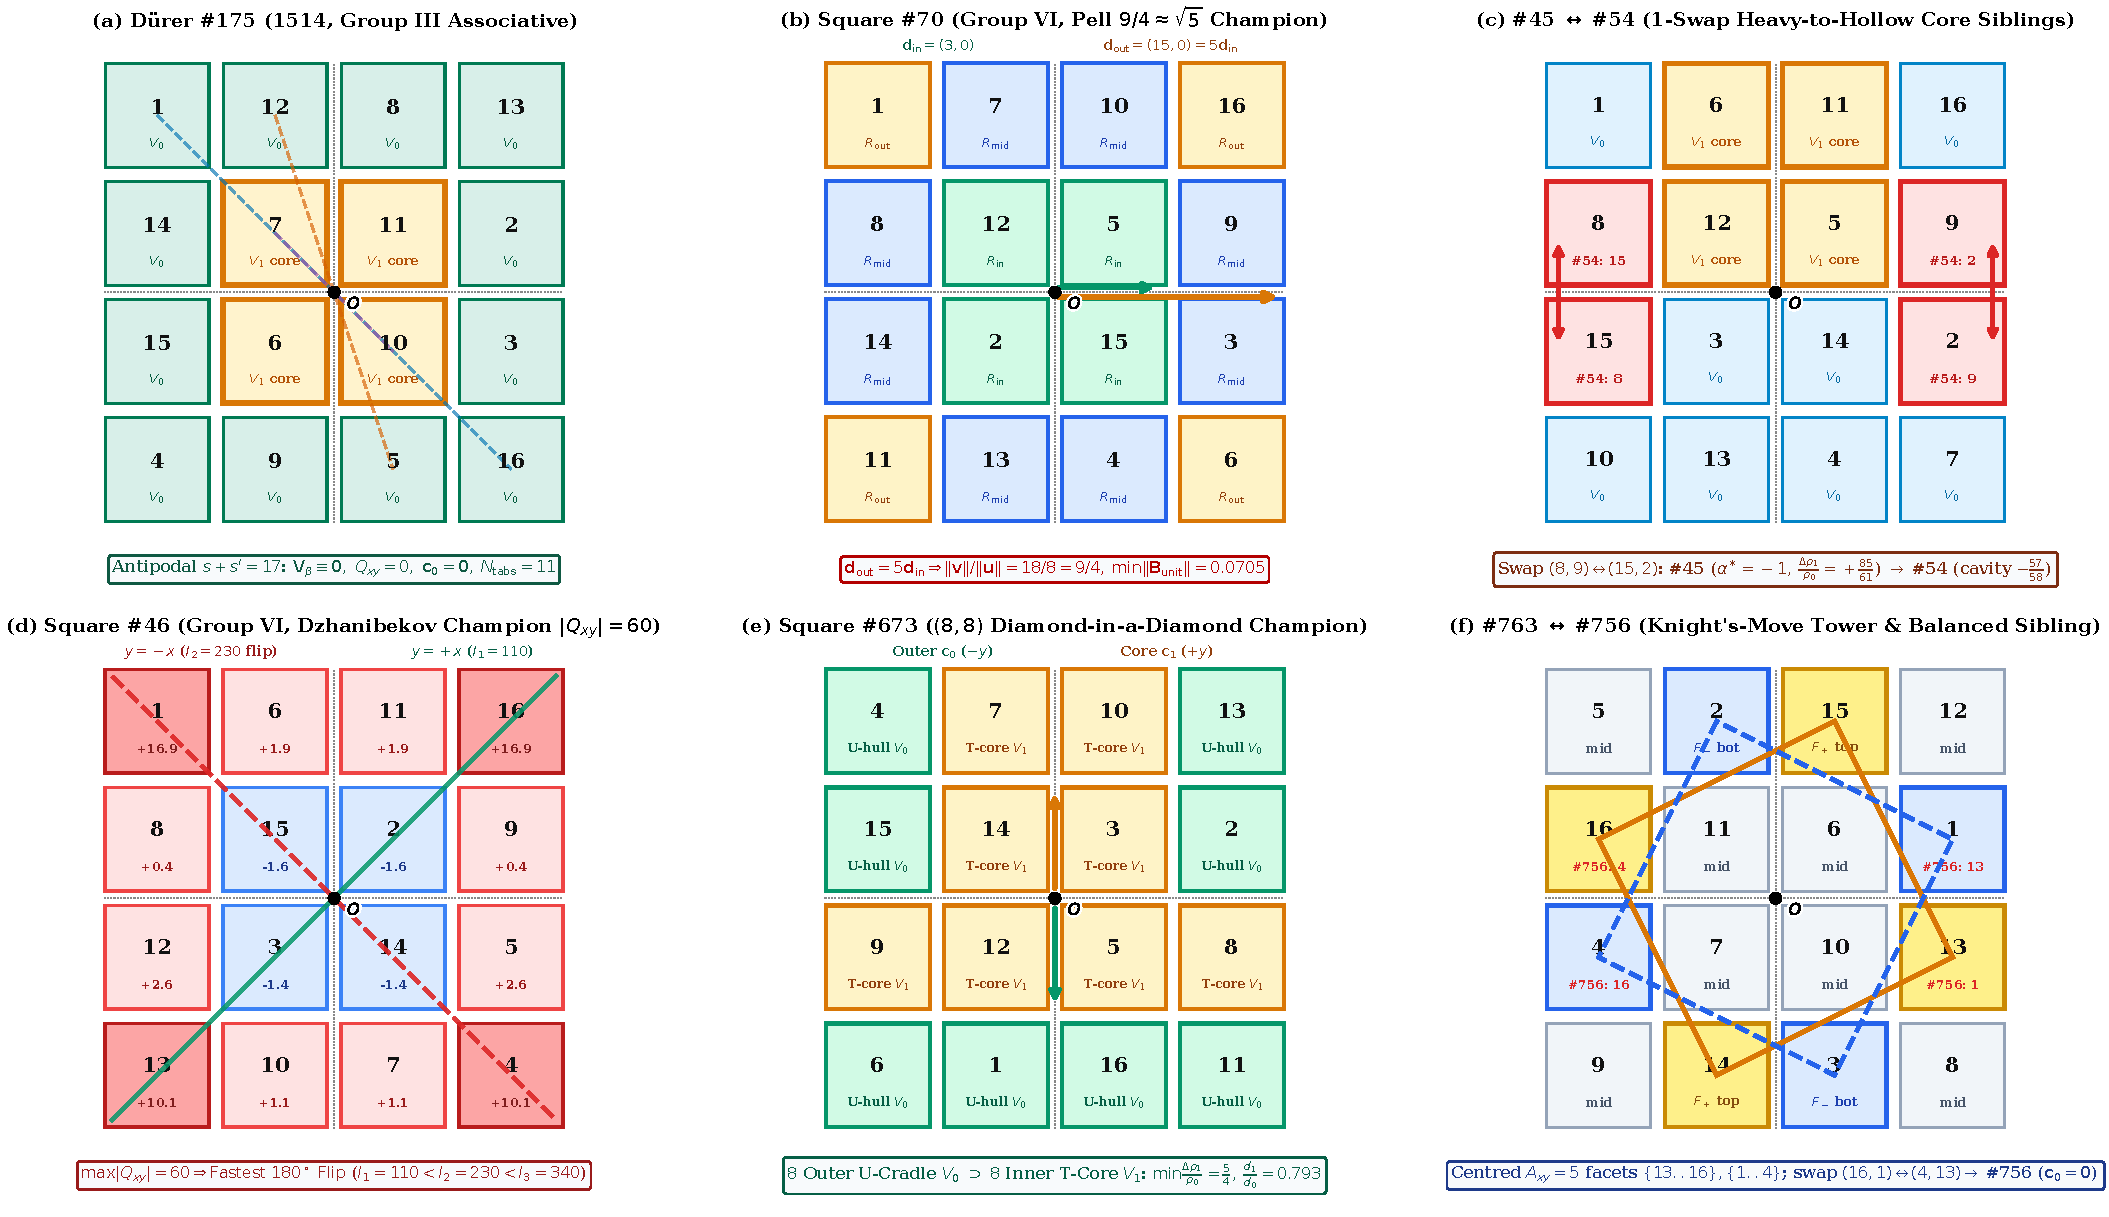
\includegraphics[width=\textwidth]{figures/fig_hero_squares_gallery.pdf}
\caption{Visual anatomy of the six flagship order-four magic squares across Sections~\ref{sec:vectors}--\ref{sec:stacking}. (a)~D\"urer's associative square \#175 (1514, Group~III), whose antipodal pairs sum to $17$ across $O$, partitioning into $12$ outer hull vertices $V_0$ and $4$ inner core vertices $V_1=\{6,7,10,11\}$. (b)~Square \#70 (Group~VI), coloured by concentric rings $R_{\mathrm{in}},R_{\mathrm{mid}},R_{\mathrm{out}}$, where parallel ring dipoles $\mathbf d_{\mathrm{out}}=(15,0)=5\mathbf d_{\mathrm{in}}$ achieve the fundamental Pell ratio $\|\mathbf v\|/\|\mathbf u\|=18/8=9/4\approx\sqrt{5}$. (c)~Square \#45 ($\kappa=+9$, inverse-radial root $\alpha^*=-1$, heavy core $\Delta\rho_1/\rho_0=+85/61$), where swapping the single outer border pair $(8,9)\leftrightarrow(15,2)$ between rows~$2$ and~$3$ yields sibling \#54 with the same $(V_0,V_1)=(10,6)$ vertex partition but a nearly hollow core cavity ($\Delta\rho_1/\rho_0=-57/58$). (d)~Square \#46 (Group~VI), shaded by cell quadrupole contribution $z_{ij}x_jy_i$, attaining the global maximum $|Q_{xy}|=60$ ($I_1=110<I_2=230<I_3=340$) and fastest $180^\circ$ Dzhanibekov flip about $y=-x$. (e)~Square \#673 (Group~VI), whose $8$ outer vertices form a U-cradle $V_0$ enclosing an $8$-vertex inverted-T core $V_1$, achieving the minimum solid excess density $\Delta\rho_1/\rho_0=5/4$. (f)~Square \#763 (Group~VI), whose centred $2\times1$ knight's-move facets $\{13,14,15,16\}$ and $\{1,2,3,4\}$ lock into an area-$5$ mirror-twin tower, and whose single border-pair swap $(16,1)\leftrightarrow(4,13)$ produces the naturally balanced solid \#756 ($\mathbf c_0=\mathbf 0$).}
\label{fig:hero-squares}
\end{figure}

\begin{enumerate}
\item \textbf{Radial spoke sculptures and balance wheels from the origin (\Cref{sec:vectors}).} Scaling 3D spoke lengths by $L_{ij}=R_{ij}(\lambda)^\beta$ is mechanically dual to weighting natural vectors $\mathbf p_{ij}(\lambda)$ by $w_{ij}=R_{ij}(\lambda)^{\beta-1}$ (\Cref{prop:reciprocity}). In 3D (\Cref{thm:3d-power}, \Cref{fig:origin-vectors-3d}), cubic spokes ($\beta=3$) have a strictly vanishing vertical resultant $(\mathbf V_3)_z=0$ for every semi-magic square, while on the unit sphere $S^2$ ($\beta=0$) every order-four square admits strictly positive minimum-variance weights $\mathbf w^*(S)>\mathbf 0$ restoring $\sum w_{ij}^*\hat{\mathbf p}_{ij}=\mathbf 0$. In the grid plane (\Cref{thm:three-ring}, \Cref{fig:ring-vectors}), decomposing $A_4$ into three concentric rings of radii $r_1=\sqrt{2}/2$, $r_2=\sqrt{10}/2$, and $r_3=3\sqrt{2}/2$ proves that unit-length planar spokes ($\alpha=0$) can never balance because $r_2/r_1=\sqrt{5}\notin\Q$; instead, $\min_{\mathcal M_4}\|\mathbf B_{\mathrm{unit}}(S)\|_2=\frac{18\sqrt{10}}{5}-8\sqrt{2}\approx0.0705$ is governed by the Pell convergent $9/4\approx\sqrt{5}$ on eight Group~VI squares led by \#70 (\Cref{fig:hero-squares}(b)), while $204$ squares with parallel dipoles $\mathbf d_{\mathrm{out}}=\kappa\mathbf d_{\mathrm{in}}$ admit a second power-law root $\alpha^*(\kappa)\ne1$, including $25$ at $\alpha^*=-1$ (\#45, \Cref{fig:hero-squares}(c)) and $25$ at $\alpha^*=+3$ (\#286; \Cref{cor:planar-power-roots}).

\item \textbf{Three-dimensional rotation: symmetric-top precession and Dzhanibekov flips (\Cref{sec:dynamics}).} For equal point masses at $\mathbf p_{ij}(\lambda)$, vanishing of the first moments makes the inertia tensor about $O$ strictly axisymmetric with universal ratio $I_\perp(\lambda)/I_{zz}=\frac12(1+\lambda^2(n^2+1))$ (\Cref{thm:rotor}, \Cref{fig:precession}(a)): every point-weighted gem passes through an exact \emph{spherical-top transition} at $\lambda_{\mathrm{iso}}=(n^2+1)^{-1/2}$ ($1/\sqrt{17}\approx0.2425$ at $n=4$) and a $9:1$ closed-orbit prolate regime at $\lambda=1$. Conversely, entry-weighted masses $m_{ij}=s_{ij}$ (\Cref{thm:quadrupole-split}) split the horizontal principal moments by $2|Q_{xy}(S)|=2|\sum z_{ij}x_jy_i|$ along $y=\pm x$ and couple the vertical products of inertia to $\mathbf V_3(S;\lambda)$, triggering $180^\circ$ Dzhanibekov flips on $824$ of the $880$ squares (led by \#46 at $|Q_{xy}|=60$, \Cref{fig:hero-squares}(d) and \Cref{fig:precession}(b--d)).

\item \textbf{Restoring solid, skeletal, and thin-shell balance via ``diamond-in-a-diamond'' layers, complete $K_N$ networks, and papercraft nets (\Cref{sec:nested}).} Casting a uniform solid $\mathcal G_0(S)=\conv P_S$ shifts $\mathbf c_0(S)$ away from $O$ on $829$ of the $880$ squares, leaving $51$ naturally balanced solids ($48$ associative plus Group~VI squares \#86, \#739, and \#756; \Cref{prop:51-balanced}). Peeling $\mathcal G_0(S)\supset\mathcal G_1(S)$ (\Cref{prop:opposition}) yields $35$ two-density balanced solids (\Cref{thm:diamond-balance}, \Cref{fig:nested-diamonds}): $33$ with a denser inner core (led by \#673 at $\Delta\rho_1/\rho_0=5/4$, \Cref{fig:hero-squares}(e)) and $2$ (\#123 and \#54, \Cref{fig:hero-squares}(c)) where volumetric simplex weighting pulls $\mathbf c_0$ to the same side of $O$ as $\mathbf c_1$, requiring a lighter or nearly hollow core cavity. For skeletal and sheet fabrications (\Cref{subsec:wireframes-nets}, \Cref{fig:wireframes-nets}), the complete $\binom{N}{2}$-rod network $K_N$ with equal-mass rods has $\mathbf c(K_N)=\mathbf 0$ and $\Sigma_{\mathrm{rods}}=\frac{2N-3}{3(N-1)}\Sigma(\lambda)=\frac{29}{45}\Sigma(\lambda)$ at $n=4$ (\Cref{thm:complete-network}), tuning inner-to-outer rod diameters $d_1/d_0$ balances $158$ Group~VI wireframes at $\lambda=1$ ($164$ at $\lambda=0.20$), and every gem unfolds along a breadth-first dual spanning tree into a non-overlapping 2D papercraft net with $N_{\mathrm{tabs}}=f_0-1$ glue tabs (\Cref{prop:papercraft-net}).

\item \textbf{Mirror-twin facet locking and chiral vertical towers (\Cref{sec:stacking}).} While only $124$ of the $880$ gems have parallel top and bottom facets on the \emph{same} gem, the half-turned complement $S^*=r^2\overline S$ satisfies $\mathcal G_\lambda(S^*)=-\mathcal G_\lambda(S)$ (\Cref{thm:mirror-tower}), pairing every upper facet $F_+\subset\mathcal G_\lambda(S)$ with a congruent parallel lower facet $-F_+\subset\mathcal G_\lambda(S^*)$. Alternating unrotated translates of $\mathcal G_\lambda(S)$ and $\mathcal G_\lambda(S^*)$ along centrally symmetric vertical-axis facets forms a zero-drift vertical tower for $48$ gems (\Cref{prop:knights-move}, \Cref{fig:mirror-stacking}), led by $17$ gems with area-$5$ centred knight's-move square facets such as chiral Group~VI gem \#763 (\Cref{fig:hero-squares}(f), \Cref{rem:chirality}).
\end{enumerate}

Every theorem and census table in this paper is certified in exact integer and rational arithmetic (\texttt{fractions.Fraction}) by \texttt{anc/verify\_paper\_c.py} (\Cref{sec:appendix}), and all five mechanical regimes can be explored in real time in the companion interactive browser visual essay (\texttt{web/index.html}).

\paragraph{Conventions, indexing, and relation to companion work.}
Let $A_n=\{(x_j,y_i):0\le i,j<n\}$ denote the centred grid \eqref{eq:coords}, let $a_n=(n^2-1)/12$ and $b_n=(n^4-1)/12=(n^2+1)a_n$ denote the marginal variances of $x_j$ and $z_{ij}$, and let the dihedral group $D_4=\langle r,h\rangle$ (with $90^\circ$ rotation $r$ and horizontal/vertical reflections $h,v$) act on arrangements together with the complement involution $\tau(S)=\overline S=(N+1)\mathbf 1-S$. An arrangement $S$ is \emph{associative} (Dudeney's Group~III of $48$ squares at $n=4$, including D\"urer's \#175) if $r^2 S=\overline S$, i.e.\ $z(-x,-y)=-z(x,y)$, and belongs to Dudeney's \emph{Group~VI} ($304$ squares at $n=4$) if $\overline S$ equals $hS$ or $vS$, inducing a $180^\circ$ half-turn symmetry ($C_2\subset SO(3)$) of $\mathcal G_\lambda(S)$ in $\R^3$. Companion preprints \cite{mathewson2026gems,mathewson2026moments} catalogue the static polyhedral combinatorics and bivariate Prouhet--Tarry--Escott moment hierarchy of semi-magic squares; the present paper is self-contained. Order-four magic squares are numbered $\#1,\dots,\#880$ by their 1-based position in Fr\'enicle's standard list (\texttt{anc/squares880.txt}); Tables~\ref{tab:two-density} and \ref{tab:knights-move} also list the 0-based index ($\#0=\#1-1$).
